\documentclass[pdf, handout]{beamer}
\mode<presentation>{\usetheme{Warsaw}}
\setbeamertemplate{headline}{}
\setbeamertemplate{section page}[mine]
\setbeamertemplate{footline}[frame number]

\title{Valuation of Options - part 1}
\subtitle{Quantitative Finance}
\author{Tilburg University}
\institute{Ramon van den Akker}
\date{}

\usepackage{array}
\usepackage{multirow}
\usepackage{amsmath}
\usepackage{multicol}
\usepackage{subfigure}
\usepackage{graphicx}
\usepackage{pstricks}
\input{commands.txt}
\newcommand{\Var}{\operatorname{Var}}
\renewcommand{\epsi}{\varepsilon}
\newcommand{\argmin}{\mathop{\mathrm{arg\,min}}}
\newcommand{\rank}{\operatorname{rank}}
\renewcommand{\kansp}{\mathbb{P}}
\renewcommand{\calF}{\mathcal{F}}
\newcommand{\e}{\operatorname{e}}
\newcommand{\Bin}{\operatorname{Bin}}
\newcommand{\kbin}{\operatorname{b}}
\newcommand{\lin}{\operatorname{lin}}
\newcommand{\kansq}{\mathbb{Q}}
%\newarrow{hulp}{<}{filler}{middle}{filler}{head}
\DeclareMathOperator*\ster{*} \DeclareMathOperator*\argmax{argmax}
\usepackage{color}
\AtBeginSection{\frame{\sectionpage}}
%\AtBeginSubsection{\frame{\subsectionpage}}
\newtranslation[to=greek]{Section}{En'othta}
\newtranslation[to=greek]{Subsection}{Upoen'othta}
\defbeamertemplate{section page}{mine}[1][]{%
  \begin{centering}
    {\usebeamerfont{section name}\usebeamercolor[fg]{section name}#1}
    \vskip1em\par
    \begin{beamercolorbox}[sep=12pt,center]{part title}
      \usebeamerfont{section title}\insertsection\par
    \end{beamercolorbox}
  \end{centering}
}
\defbeamertemplate{subsection page}{mine}[1][]{%
  \begin{centering}
    {\usebeamerfont{subsection name}\usebeamercolor[fg]{subsection name}#1}
    \vskip1em\par
    \begin{beamercolorbox}[sep=8pt,center,#1]{part title}
      \usebeamerfont{subsection title}\insertsubsection\par
    \end{beamercolorbox}
  \end{centering}
}

%%%%%%%%%%%%%%%%%%%%%%%%%%%%%%%%%%%%%%%%%%%%%%%%%%%%%%%%%%%%%%%%%%%%%%%%%%%
\begin{document}
\begin{frame}
\titlepage
\end{frame}

\section{Introduction}

\begin{frame}{Options (quick recap)}
\textbf{Call option} 
\begin{itemize}
\item contract between buyer (option holder) and seller (option writer)
\item contract offers buyer \emph{right} (but \emph{not obligation}!) to \emph{buy}  specified security (or other \emph{underlying financial asset})  at \emph{specific} date (\emph{maturity/expiration date}) or during a specified period of time at  \emph{agreed upon price} (\emph{strike price})
\end{itemize}
\textbf{Put option} 
\begin{itemize}
\item analogous definition; but put offers buyer right to \emph{sell}
\end{itemize}
\textbf{Remarks}
\begin{itemize}
\item As a put or call provides its buyer a right and not an obligation, the contract has a (positive) price.
\item Please note that the seller (writer) of the contract has the obligation to sell (call) or buy (put) in case the option is exercised by the buyer.
\end{itemize}
\end{frame}

\begin{frame}{Options (quick recap)}
\textbf{Underlying asset:}
\begin{itemize}
\item stock, index, ETF, interest rate(s), real estate, etc.
\end{itemize}
\textbf{Exercising the option:}
\begin{itemize}
\item \emph{European (style) options}: option can only be exercised \emph{at expiration date}
\item \emph{American}: option can be exercised \emph{at any time between
purchase and expiration date}
\item (there also exist \emph{Asian}, \emph{Bermudan} and \emph{Canary} versions; all these names have nothing to do with geographical locations)
\item typically: options on indices and interest rates are European style, while options on (individual) stocks and ETFs are American style
\end{itemize}
\textbf{Further terminology:}
\begin{itemize}
\item \emph{strike price} is a.k.a. \emph{exercise price}
\item final date for exercising option: \emph{maturity} or \emph{expiration date}
\end{itemize}
\end{frame}
%
\begin{frame}{Options (quick recap)}
\textbf{Remarks:}
\begin{itemize}
\item options are traded on exchanges, in Over-The-Counter markets, and in bespoke contracts (investment banks)
\item this course focuses on European style options (on stocks, indices, ETFs); see MSc QFAS for American style options and options on interest rates
\item options are examples of \emph{financial derivatives} which are contracts that are defined in terms of underlying asset which is traded on financial market
\end{itemize}
\end{frame}

\begin{frame}{Options (quick recap)}
\textbf{Exercise}\\ Check the following formulas for the payoff at maturity $T$.
\begin{itemize}
\item European call option with strike price $K$:  $C_T=\max\{ S_T -K , 0\}$
\item European put option with strike price $K$:  $C_T=\max\{ K-S_T  , 0\}$
\end{itemize}
\vspace{.25cm}
We will often use the following options that are defined by their pay-off:
\begin{itemize}
\item European digital (binary) call option with strike price $K$:  $C_T=1\{ S_T -K \geq 0\}$
\item European digital (binary) put option with strike price $K$:  $C_T=1\{ K -S_T \geq 0\}$
\end{itemize}
Please recall that $1\{ x\leq K\} =1$ if $x\leq K$ and 0 otherwise.
\\ \vspace{.5cm}
Note that can write all these payoffs as a function of $S_T$, i.e. $C_T = g(S_T)$.
\end{frame}


\begin{frame}{Options (quick recap)}
As an example, we will consider European call and put options on the AEX-index at September 3, 2021. 
\begin{figure}
\includegraphics[width=1\textwidth]{AEX}
\end{figure}
\end{frame}

\begin{frame}{Options (quick recap)}
As an example, we will consider European call and put options, on the AEX-index at September 3, 2021, with expiration date in December 2022.
\begin{figure}
\includegraphics[width=1\textwidth]{AEX-opties}
\end{figure}
\end{frame}

\begin{frame}{Main problems}
\textbf{Valuation/pricing} \\
What is the `fair' price of an option and how does it evolve over time? This is an important question for:
\begin{itemize}
\item investors/traders
\begin{itemize}
\item to identify that you don't pay too much
\item to make money in case you think the market price is wrong
\end{itemize}
\item financial institutions
\begin{itemize}
\item who need to calculate price for selling
OTC-options (or to price `embedded' options)
\item who need to perform risk management on
portfolios that contain options 
\end{itemize}
\end{itemize}
\vspace{.5cm}
\emph{Remark}: later on we will also discuss \textbf{hedging}.
\end{frame}

\begin{frame}{Main problems - valuation}
\begin{itemize}
\item we are interested in (fair) price $C_t$, for $t\in [0,T)$, of (European) option with payoff $C_T=f(T,S_T)$ at maturity $T$
\item we will learn three methods to determine `fair price' (using specified continuous-time model for financial market):
\begin{itemize}
\item Black-Scholes Partial Differential Equation
\item risk-neutral pricing
\item pricing kernel
\end{itemize}
\item in particular: you will derive the famous Black-Scholes price for European put option with maturity $T$ and strike $K$:
{%\small
\begin{align*}
C_t&=p(S_t,T-t,K,r,\sigma)= K\e^{-r (T-t)} \Phi(-d_2) -    S_t  \Phi(-d_1)
\\
d_1&=\frac{ \log\left(\frac{S_t}{K}\right) + \left( r+ \frac{\sigma^2}{2}\right) (T-t)}{ \sigma \sqrt{T-t}}, \quad d_2=d_1-\sigma \sqrt{T-t},
\end{align*}
}
\begin{itemize}
\item does not depend on $\mu$!
\end{itemize}
\end{itemize}
\end{frame}
%
\begin{frame}{Black-Scholes formula}
\begin{figure}
\includegraphics[width=0.84\textwidth]{BSM}
\end{figure}
\begin{itemize}
\item in 1973 Fisher Black and Myron Scholes published paper
`The Pricing of Options and Corporate Liabilities'  and Robert Merton
published `Theory of Rational Option Pricing'
\item Merton and Scholes received Nobel Memorial Prize in Economic Sciences in 1997 (Black died in 1995)
\end{itemize}
\end{frame}

\begin{frame}{Arbitrage}
All pricing methods we discuss rely on insisting that arbitrage opportunities do/should not
exist.

\begin{definition}
If it is possible to find an admissible self-financing trading strategy with value process $V$ such that, for some  $T>0$, we have
$V_0\leq 0$ and
\[
\mathbb{P}( V_T< 0 )=0 \text{ and }  \mathbb{P}( V_T> 0 )>0,
\]
then we say that an arbitrage opportunity exists.
\end{definition}
\textbf{Remarks:}
\begin{itemize}
\item in QF you are allowed to ignore `admissible': this condition rules out 'doubling strategies'. A sufficient condition for admissibility: $\mathbb{E}V_t^2<\infty$ for all $t\in[0,T]$, 
where $V_t$ denotes the porfolio value of the self-financing strategy
\end{itemize}

%\begin{figure}
%
\includegraphics[angle=270,width=0.3\textwidth]{gordon-gekko.eps}
%\end{figure}
\end{frame}

\section{Toy model}

\begin{frame}{Motivation}
First we discuss a very simple discrete time model and discuss pricing of options under assumption that arbitrage opportunities do not exist.
We discuss two methods:
\begin{itemize}
\item pricing by replication
\item risk-neutral pricing
%\item pricing kernel
\end{itemize}
Later on we will discuss their continuous-time analogues.
Although the math gets more complicated, 
the underlying ideas are the same!
\end{frame}


\begin{frame}{Model for financial market}
\begin{itemize}
\item two states-of-the-world: $\Omega=\{ \text{``up''},\text{``down''}\}$
\item two assets: risky asset $S$ and riskless asset $B$
\begin{itemize}
\item $B_1(\text{``up''})=B_1(\text{``down''})=B_1>0$
\item for
\[
S_1(\omega)=\left\{
              \begin{array}{ll}
                s_u, & \hbox{ if } \omega=\text{``up''} \\
                s_d, & \hbox{ if }\omega=\text{``down''}
              \end{array}
            \right.
\]
we assume 
$0<s_d<s_u$
\end{itemize}
\item  probability of state ``up'' is $p\in(0,1)$, i.e. $\mathbb{P}(\text{``up''})=p$
\end{itemize}
\begin{figure}
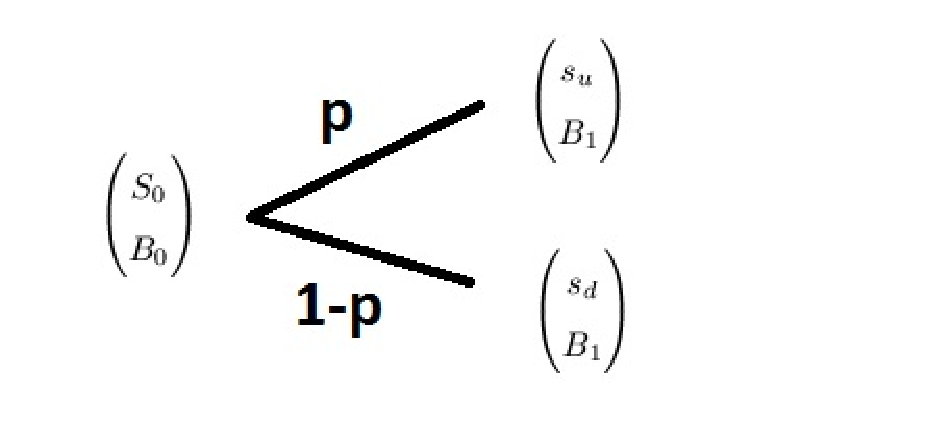
\includegraphics[width=0.75\textwidth]{1period-1.eps}
\end{figure}
\end{frame}

\begin{frame}{No arbitrage}
\textbf{Theorem} 
There are no arbitrage opportunities in our financial market if and only if 
\[
0<\frac{s_d}{s_0}<\frac{B_1}{B_0}<\frac{s_u}{s_0}.
\]
\textbf{Proof} \\
`$\Rightarrow$':  exercise \\
 `$\Leftarrow$':  this will follow from our proofs of other results (verify!)
\end{frame}

\begin{frame}{What's the price of an option in this market?}
\begin{itemize}
\item now consider European option with payoff
\[
C_1(\omega)=\left\{
              \begin{array}{ll}
                c_u, & \hbox{ if }\omega=\text{``up''} \\
                c_d, & \hbox{ if }\omega=\text{``down''}
              \end{array}
            \right.
\]
\begin{itemize}
\item for call:  $c_u=\max\{s_u-K,0\}$ and $c_d=\max\{s_d-K,0\}$
\end{itemize}
\item what is price at $t=0$ for call?
\end{itemize}
\begin{figure}
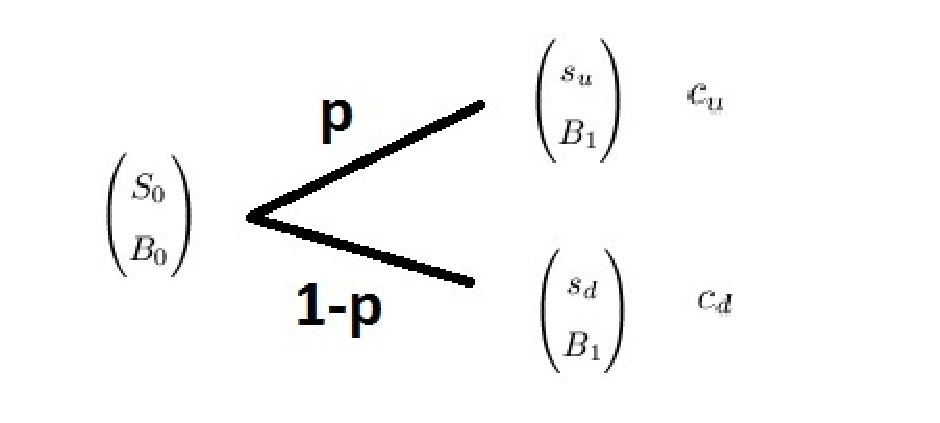
\includegraphics[width=0.85\textwidth]{1period-2.eps}
\end{figure}
\end{frame}

\begin{frame}{Method 1: pricing by replication}
\begin{itemize}
\item construct portfolio $V$ with $V_1(\omega)=C_1(\omega)$ for all $\omega$
\begin{itemize}
\item as portfolio generates exactly the same pay-offs as option does (for all states-of-the-world), the portfolio is called \emph{replicating} portfolio
\item Why? As there are no intermediate cashflows, we must have $C_0 = \phi S_0 + \psi B_0$. Otherwise
we would create arbitrage opportunities. So via the replicating portfolio we find no-arbitrage price of option
\end{itemize}
\item notice that we have to determine $\phi$ and $\psi$ such that
\begin{align*}
c_u&= \phi s_u + \psi B_1 \\
c_d&= \phi s_d + \psi B_1
\end{align*}
which yields
\[
\phi=\frac{ c_u -c_d}{s_u-s_d} \text{ and } \psi=\frac{c_d s_u - s_d c_u}{B_1(s_u-s_d)}
\]
\item price of option (at $t=0$):
\[
C_0=\phi S_0 + \psi B_0
\]
\end{itemize}
\end{frame}

\begin{frame}{Method 2: risk-neutral pricing}
\textbf{Motivation}
\begin{itemize}
\item
people would like to have pricing formula of the form:
\[
\frac{A_0}{B_0} = \mathbb{E}\left[ \frac{A_1}{B_1} \right]  
\]
for all assets $A$, i.e. price equals expected discounted cashflows
\item note that
\[
\frac{A_0}{B_0} = \mathbb{E}\left[ \frac{A_1}{B_1} \right] \quad \Longleftrightarrow\quad
 \mathbb{E}\left[ \frac{A_1}{A_0} \right] =\frac{B_1}{B_0}
\]
\item however, already for $A=S$ this almost never holds true in real
financial markets:
\[
 \mathbb{E}\left[ \frac{S_1}{S_0} \right] =\frac{B_1}{B_0},
\]
would mean that expected (gross) return on stock is same as
return on riskless asset
\end{itemize}
\end{frame}

\begin{frame}{Intermezzo:  a biased coin can save the day} 
\begin{itemize}
\item
Suppose we throw a \emph{fair} coin, $\Omega=\{H,T\}$, and you get
pay-off $X=1$ if $\omega=H$ and $X=0$ if $\omega=T$
\item the price of entering this game is 0.3 (given)
\item (for some reason) we want to have the identity
\[
\text{price} = \mathbb{E}[ X] = \text{Prob}(\{H\})
\]
\item as the coin is fair the equation does not hold true if we use the true, ``real-world'',  probability measure ($0.3\neq 0.5)$
\item however: we can just create \emph{artificial} probability measure
$\mathbb{Q}$ with $\mathbb{Q}(\{H\})=0.3$, which does lead to
\[
\text{price} = \mathbb{E}_{\mathbb{Q}}[X]
\]
\end{itemize}
\end{frame}

\begin{frame}{Method 2: risk-neutral pricing}
\begin{itemize}
\item  people would like to have pricing formula of the form:
\[
\frac{A_0}{B_0} = \mathbb{E}\left[ \frac{A_1}{B_1} \right]\quad   
\Longleftrightarrow\quad
 \mathbb{E}\left[ \frac{A_1}{A_0} \right] =\frac{B_1}{B_0}\quad (\star)
\]
for all assets $A$
\item if we use ``real-world'' probabilities then this identity will
typically not hold for $A=S$
\item could we repair identity by using artificial probability measure $\mathbb{Q}$ instead of ``real-world'' measure $\mathbb{P}$?
\item solving
\[
\frac{S_0}{B_0}=\mathbb{E}_{\mathbb{Q}}
\left[ \frac{S_1}{B_1}\right] = q \frac{s_u}{B_1}  +(1-q) \frac{s_d}{B_1}
\]
yields
\[
q=\frac{\frac{B_1}{B_0}-\frac{s_d}{s_0}    }{ \frac{s_u}{s_0}-\frac{s_d}{s_0}  }
\]
\item if $q\in [0,1]$ then we indeed have found 
artificial probability measure for which $(\star)$ is true by construction
(for $A=B$ the identity is trivial)
\end{itemize}
\end{frame}

\begin{frame}{Method 2: risk-neutral pricing}
Recall earlier theorem: there is no arbitrage if and only if
\[
0<\frac{s_d}{s_0}<\frac{B_1}{B_0}<\frac{s_u}{s_0}
\]
which occurs exactly if $q\in (0,1)$. So we have proved:
\\
\vspace{.3cm}
\textbf{Intermediate result} \\
The market is free of arbitrage opportunities if and only if there exists a probability measure $\mathbb{Q}$ equivalent to $\mathbb{P}$
 such that $S/B$ is a martingale under $\mathbb{Q}$, i.e.
\[ 
 \frac{S_0}{B_0} =\mathbb{E}_{\mathbb{Q}}[ \frac{S_1}{B_1} ].
\]
%\end{itemize}
\end{frame}

\begin{frame}{Method 2: risk-neutral pricing}
Terminology:
\begin{itemize}
\item As $S/B$ is martingale under $\mathbb{Q}$ we have
\[
\frac{s_0}{B_0}=\mathbb{E}_{\mathbb{Q}}\left[ \frac{S_1}{B_1}\right],
\]
which yields
\[
\frac{B_1}{B_0} =\mathbb{E}_{\mathbb{Q}} \left[ \frac{S_1}{S_0} \right] ,
\]
i.e. the expected (gross) return on the risky asset $S$, under $\mathbb{Q}$, is equal to the return/interest on the riskless asset $B$.
\item $\mathbb{Q}$ is often called ``risk-neutral measure''
\begin{itemize}
\item Please note that $\mathbb{Q}$ is \emph{artificial} measure and does not describe actual probabilities!
\end{itemize}
\item $\mathbb{Q}$ is also called \emph{equivalent martingale measure}
\end{itemize}
\end{frame}

\begin{frame}{Method 2: risk-neutral pricing}
So we have repaired the formula  $S_0/B_0 = \mathbb{E}[S_1/B_1]$, but it 
was quite a discussion.  What is the true benefit?
\begin{itemize}
\item introduce, as before, an option to the market (with payoff $C_1$ at $t=1$)
\item we already know that there is a replicating portfolio $(\phi,\psi)$ such that $V_1(\omega) =\phi S_1(\omega) + \psi B_1= C_1(\omega)$ for all $\omega$
\item and, if there are no arbitrage opportunities, $C_0=\phi S_0 + \psi B_0$
\item now note that
\begin{align*}
\mathbb{E}_{\mathbb{Q}}\left[ \frac{C_1} {B_1} \right]
=\phi \mathbb{E}_{\mathbb{Q}}\left[ \frac{S_1} {B_1} \right]
+\psi = \phi \frac{S_0}{B_0} + \psi = \frac{1}{B_0}( \phi S_0 + \psi B_0)=\frac{C_0}{B_0}, 
\end{align*}
so we can calculate for any option (or asset) its price at $t=0$ via the above identity as soon as we know $\mathbb{Q}$! There is no need to calculate 
the replicating portfolios. 
\end{itemize}
\end{frame}

\begin{frame}{Method 2: risk-neutral pricing}
\textbf{First fundamental theorem of asset pricing (for the toy model)} \\
The market is free of arbitrage opportunities if and only if there exists a probability measure $\mathbb{Q}$ equivalent to $\mathbb{P}$
 such that $A/B$ is a martingale, under $\mathbb{Q}$, for all assets $A$.
\\ \vspace{.5cm}
\textbf{Application} We can price options by applying this theorem twice:
\begin{itemize}
\item Write down model for $B$ and $S$ (without arbitrage opportunities).
\item  Apply theorem (with $A= B$ and $A=S$; note that for $A=B$ the `martingale-property' is  trivial). This yields unique $\mathbb{Q}$.  ($\star$)
\item Now introduce an option to market with payoff $C_1$. We want to set
price such that we do not create arbitrage opportunity.
\item Apply theorem again: $A/B$ should be a martingale for $A=B, S, C$. For $A=S$ we obtain unique $\mathbb{Q}$ from previous step $(\star)$. 
And $A=C$ yields
\[
C_0 = B_0 \mathbb{E}_{\mathbb{Q}}[ C_1/B_1].
\]
\end{itemize}
\end{frame}

\begin{frame}{Method 2: risk-neutral pricing}
\textbf{Proof} \\
`$\Rightarrow$':  exercise - check that we have proved this implication
(via explicit construction of $\mathbb{Q}$) \\
`$\Leftarrow$': \\
Consider portfolio $V$  with $V_1\geq 0$ and $V_1(\omega) >0$ for at least one state-of-the-world. If we prove that $V_0 > 0$, then we have shown that arbitrage opportunities do not exist. \\
Note that we have (why?!)
\begin{align*}
0 &< \mathbb{E}_{\mathbb{Q}}\left[ \frac{V_1}{B_1} \right]
=
\phi\mathbb{E}_{\mathbb{Q}}\left[ \frac{S_1}{B_1} \right] + \psi
\\ 
&= \phi \frac{S_0}{B_0} + \psi = \frac{1}{B_0}(\phi S_0 + \psi B_0)
= \frac{V_0}{B_0},
\end{align*}
which yields $V_0>0$.
\end{frame}

\begin{frame}{Toy model - concluding remarks}
For the toy model we have seen that we can price options 
by
\begin{itemize}
\item constructing a replicating portfolio
\item by using risk-neutral pricing
\end{itemize}
(and it would also be possible to introduce pricing kernels as a third method).
\\
\vspace{.5cm}
For the continuous time case we will see that exactly the same ideas are used. Unfortunately (?), the math gets a bit more difficult.
\end{frame}

\end{document}